% !TeX spellcheck = en_GB
% !TeX root = Report.tex
\phantomsection
\addcontentsline{toc}{subsection}{Case 2 - Opportunities Presented by UK Government Policy on Nuclear New Build}
\subsect{Case 2 - Opportunities Presented by UK Government Policy on Nuclear New Build}

The UK has a rich nuclear heritage and has been generating commercial quantities of power from nuclear power plants since Calder Hall opened in 1957 \cite{NDA2007}. 
The nuclear industry is one of the most heavily regulated industries in which to operate and opportunities to profit from technology are strongly coupled to the position of the government and their subsequent policy decisions. 
New nuclear build marks a recent turn-around in government policy, and private companies are now positioning themselves to profit from the infrastructure investment that is sorely needed.

UK Government policy has been largely anti-new-build since the last nuclear plant was commissioned at Sizewell B in 1992. 
This plant was envisioned to be the first of a fleet of new pressurised water reactors, but only Sizewell B was ever built \cite{WNA2014}. 
The new build supply chain has since diminished, with construction expertise and nuclear specific skills depleting.
However, opportunities to profit from nuclear technology did not diminish entirely in this period. 
The UK's ageing fleet of nuclear reactors contributed 19\% of UK electricity supply in 2012 \cite{WNA2014}.  
The French utility EDF made \pounds880m profit in 2012 from their UK nuclear operation including eight plants totalling 8.7GW capacity \cite{EDF2012}. 
Evidently there were sparse but significant opportunities in the industry prior to 2008.

Government nuclear policy has gradually evolved since privatisation of the energy industry in 1995. 
Labour’s 1997 manifesto was strongly against new nuclear \cite{Birmingham2012}. 
The 2003 Energy White Paper set targets for the reduction of carbon emissions by 60\% by 2050. 
While new nuclear build was not ruled out, it was not supported for economic reasons \cite{WP2003}. 
Against a backdrop of rapidly increasing fossil fuel prices and increasing concerns over energy security, the 2007 Energy White Paper started the public consultation on new nuclear build \cite{WP2007} resulting in the plans to promote new nuclear build in the 2008 White Paper on nuclear \cite{WP2008}.
This turnaround in Government policy opens a new era of opportunity for private companies to profit from investments in new nuclear. 
The new policy is expected to attract \pounds40bn investment by 2025 \cite{Birmingham2012}.
Eight UK sites were selected for potential development, of which five sites were successfully auctioned \cite{Birmingham2012}, as shown in Figure \ref{figure:NNB}, to three different private companies each intending to deploy a different reactor technology.
%\begin{table}[!htb]
%\caption{UK Nuclear New Build Summary}
%\label{table:NNB}
%\begin{center}
%\begin{tabular}{p{0.3\textwidth}p{0.15\textwidth}p{0.15\textwidth}p{0.28\textwidth}}
%\toprule
%\textbf{Company} 		&	\textbf{Parent Company}	& 	\textbf{Sites} 	& 	\textbf{Technology} \\ \toprule
%NNB GenCo (Nuclear New Build Generation Company)&EDF Energy & Hinkley Point \& Sizewell&Areva EPR (European Pressurized Reactor)\\
%Horizon Nuclear Power&Hitachi& Wylfa \& Oldbury& Hitachi-GE ABWR (Advanced Boiling Water Reactor)\\
%NuGeneration&Toshiba \& GDF Suez&Moorside (Sellafield)&Westinghouse AP1000\\
%\bottomrule
%\end{tabular}
%\end{center}
%\end{table}

\begin{figure}[!h]
\centering
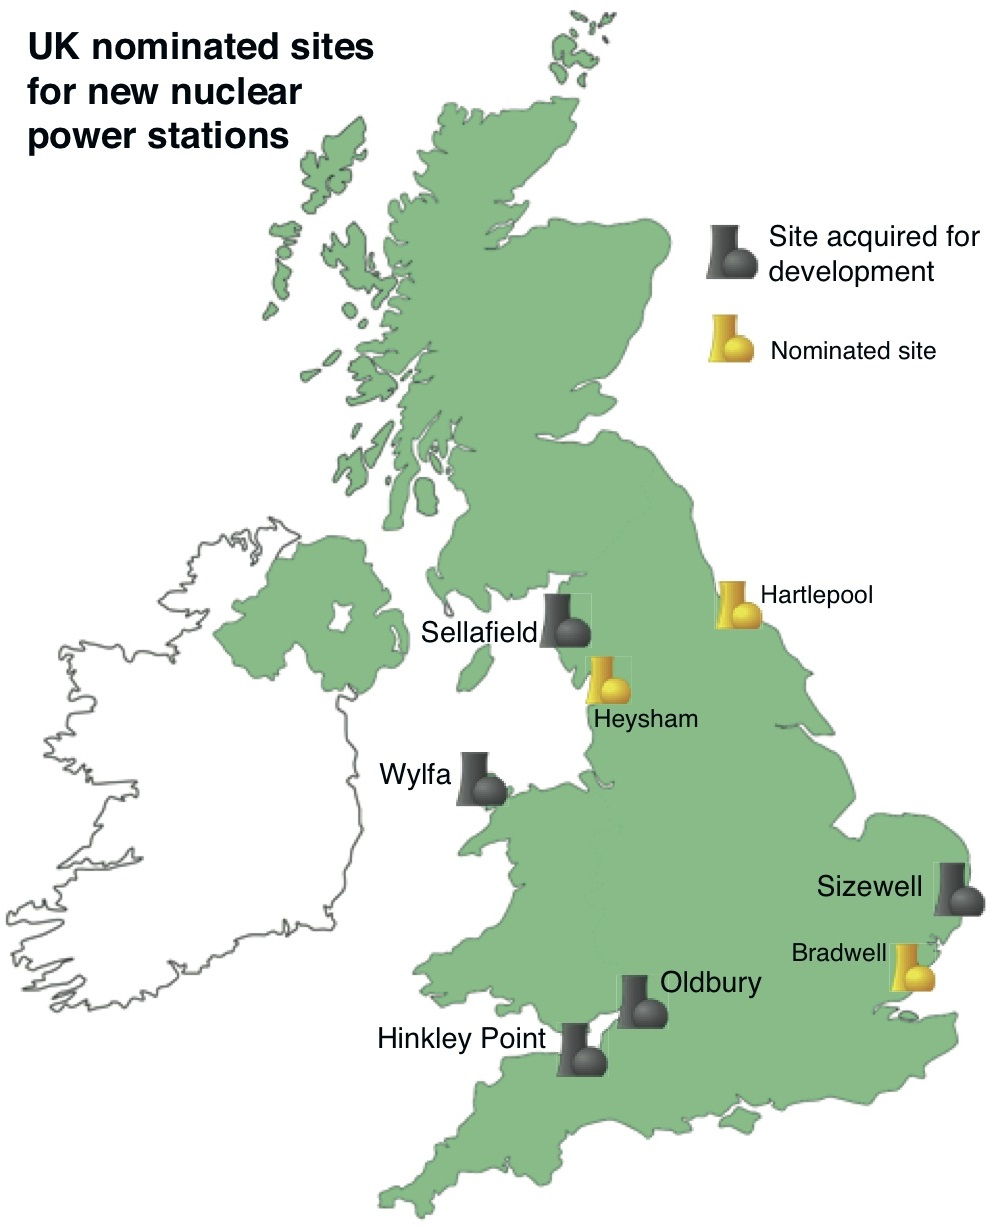
\includegraphics[width = 0.4\textwidth]{Figures/uk-nuclear-map.jpeg}
\caption{Nominated Sites for New Nuclear Build in the UK - reprinted from \cite{NAMRC}}
\label{figure:NNB}
\end{figure}

Investment in nuclear new build in the private market is difficult to secure.
A very rough estimation of daily turnover for Hinkley Point C can generate is shown in equation \eqref{CfD}, assuming a capacity of 3.2GW and a strike price of \pounds92.50 per megawatt hour.
%While a nuclear power station can generate around \pounds7m turnover per day\footnote{Hinkley Point C will be around 3.2GW capacity. The strike price is \pounds92.50 per megawatt hour (MWh) meaning that the turnover per day is $capacity \times power~price~per~hour \times hours~per~day$ or $ 3,200MW \times 92.50~\pounds/MW \times 24 = \pounds7.1m$ assuming 100\% capacity factor. This is an optimistic figure but provides some perspective.}, 
\begin{equation}
\begin{split}
\label{CfD}
Turnover &= capacity \times power~price~per~hour \times hours~per~day\\
               &= 3,200MW \times 92.50~\pounds/MWh \times 24 = \pounds7.1m
\end{split}
\end{equation}
The profit margins appear attractive, however securing investment remains difficult due to very large capital costs.
The EDF commitment to Hinkley Point C is of the order of \pounds16bn \cite{Spectator14}.
In order to stimulate investment, the 2013 Energy Act set out the final phase of the Electricity Market Reform (EMR) \cite{EnergyAct13}.
One of the major components of the reform is the introduction of contracts for difference (CfDs), which guarantee an agreed power price for renewable projects to reduce cost risk \cite{Baringa}.
CfDs are available for new nuclear projects and will help give investors in new nuclear certainty on their returns \cite{Baringa}.
The operation of CfDs is explained in Figure \ref{figure:CfD}.

\begin{figure}[!h]
\centering
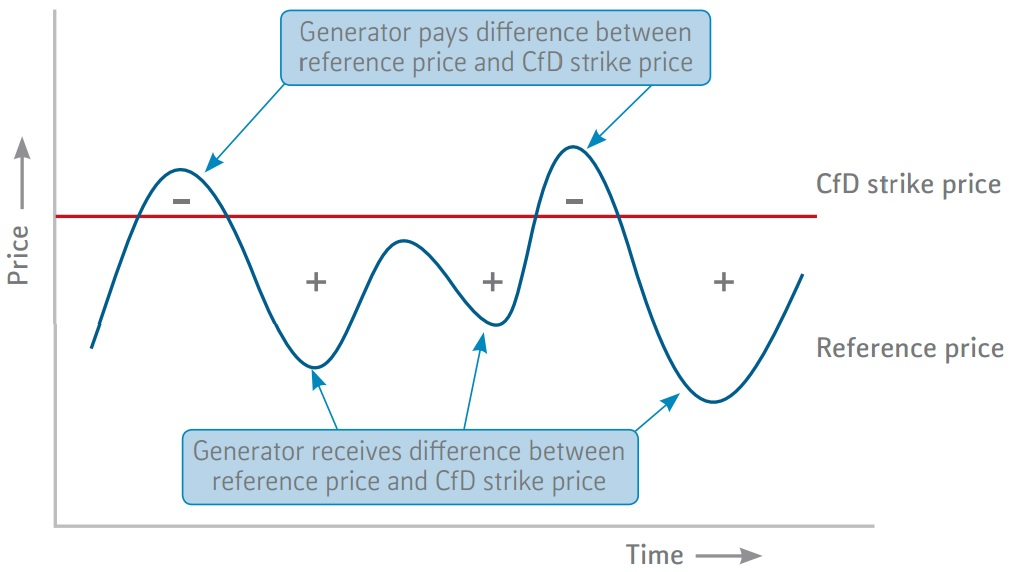
\includegraphics[width = 0.6\textwidth]{Figures/StrikePrice.jpg}
\caption{The operation of a CfD scheme - reprinted from \cite{Baringa}}
\label{figure:CfD}
\end{figure}

The first nuclear strike price was agreed for EDF's Hinkley Point project in October 2013 at \pounds92.50 per MWh, more than double the current unit price of electricity \cite{BBCnewsHinkley}. 
The spectator estimates that the Hinkley Point plant will generate pre-tax profits of between \pounds2bn - \pounds5bn per year for the duration of the 35 year contract \cite{Spectator14}.
This is a substantial return on investment given the operating profits of the big six energy companies combined was \pounds2.1bn in 2012 \cite{Spectator14}.
Cash dividends in addition to paying off the construction debt should be of the order of \pounds65bn-\pounds80bn \cite{Spectator14}.
EDF have positioned themselves in a very favourable position to profit from the opportunities in nuclear new build.
It is expected that NuGen and Horizon Nuclear Power will follow suit in the pursuance of a CfD deal.

The nuclear new build case study has shown two different impacts of governance. 
It was seen how the industry was stifled prior to 2008. 
Then the turn-around in policy shows how governance can stimulate massive investment in an otherwise dying industry.
It is clear that the new build companies and their large parent organisations stand to profit significantly from the infrastructure investment the Government requires to keep the lights on, provided adequate capital investment can be found.
